\chapter{Ostinato Model for data-driven visual network analytics}
\label{ch:ostinato}

In this chapter, we describe Ostinato Model, a process model for data-driven visual network analytics of innovation ecosystems. Ostinato Model answers \ref{objective:processmodel} and represents the main contribution of this dissertation. The Ostinato Model is developed over the series of experiments presented in Chapter~\ref{ch:experiments}. Requirements identified through the investigations and existing process models Chapter~\ref{ch:processmodels} are the key drivers in developing the Ostinato Model.  The Ostinato Model was first presented in \ref{pub:ostinato} in the context of social media studies. Here, we discuss the Ostinato model in particular in the context of investigating innovation ecosystems. This chapter is a revised version of a section in \ref{pub:ostinato}.

In music, the word \emph{ostinato} refers to both a repeating musical pattern as well as a composition that contains a repeating musical pattern. Like the repeated rhythms and melodies in Ravel's Bolero in Figure~\ref{fig:bolero-ostinato} or distinctive in post-rock\footnote{Categorizing music is  debatable at best. However, music that falls under the post-rock category has been playing in the earphones of the author of this dissertation for hours and hours while conducting the investigations and writing this manuscript. For a sample, please refer to \href{https://www.youtube.com/watch?v=fD2HgZMdxOI}{Magyar Posse}.}--small innovations are explored with each iteration, and some are incorporated into the melodic narrative--we apply the musical concept of ostinato to a cycle of user-centric exploration and automation that builds transparency of authorship for evidence-based decision making.

\begin{figure}[htb]
\centering
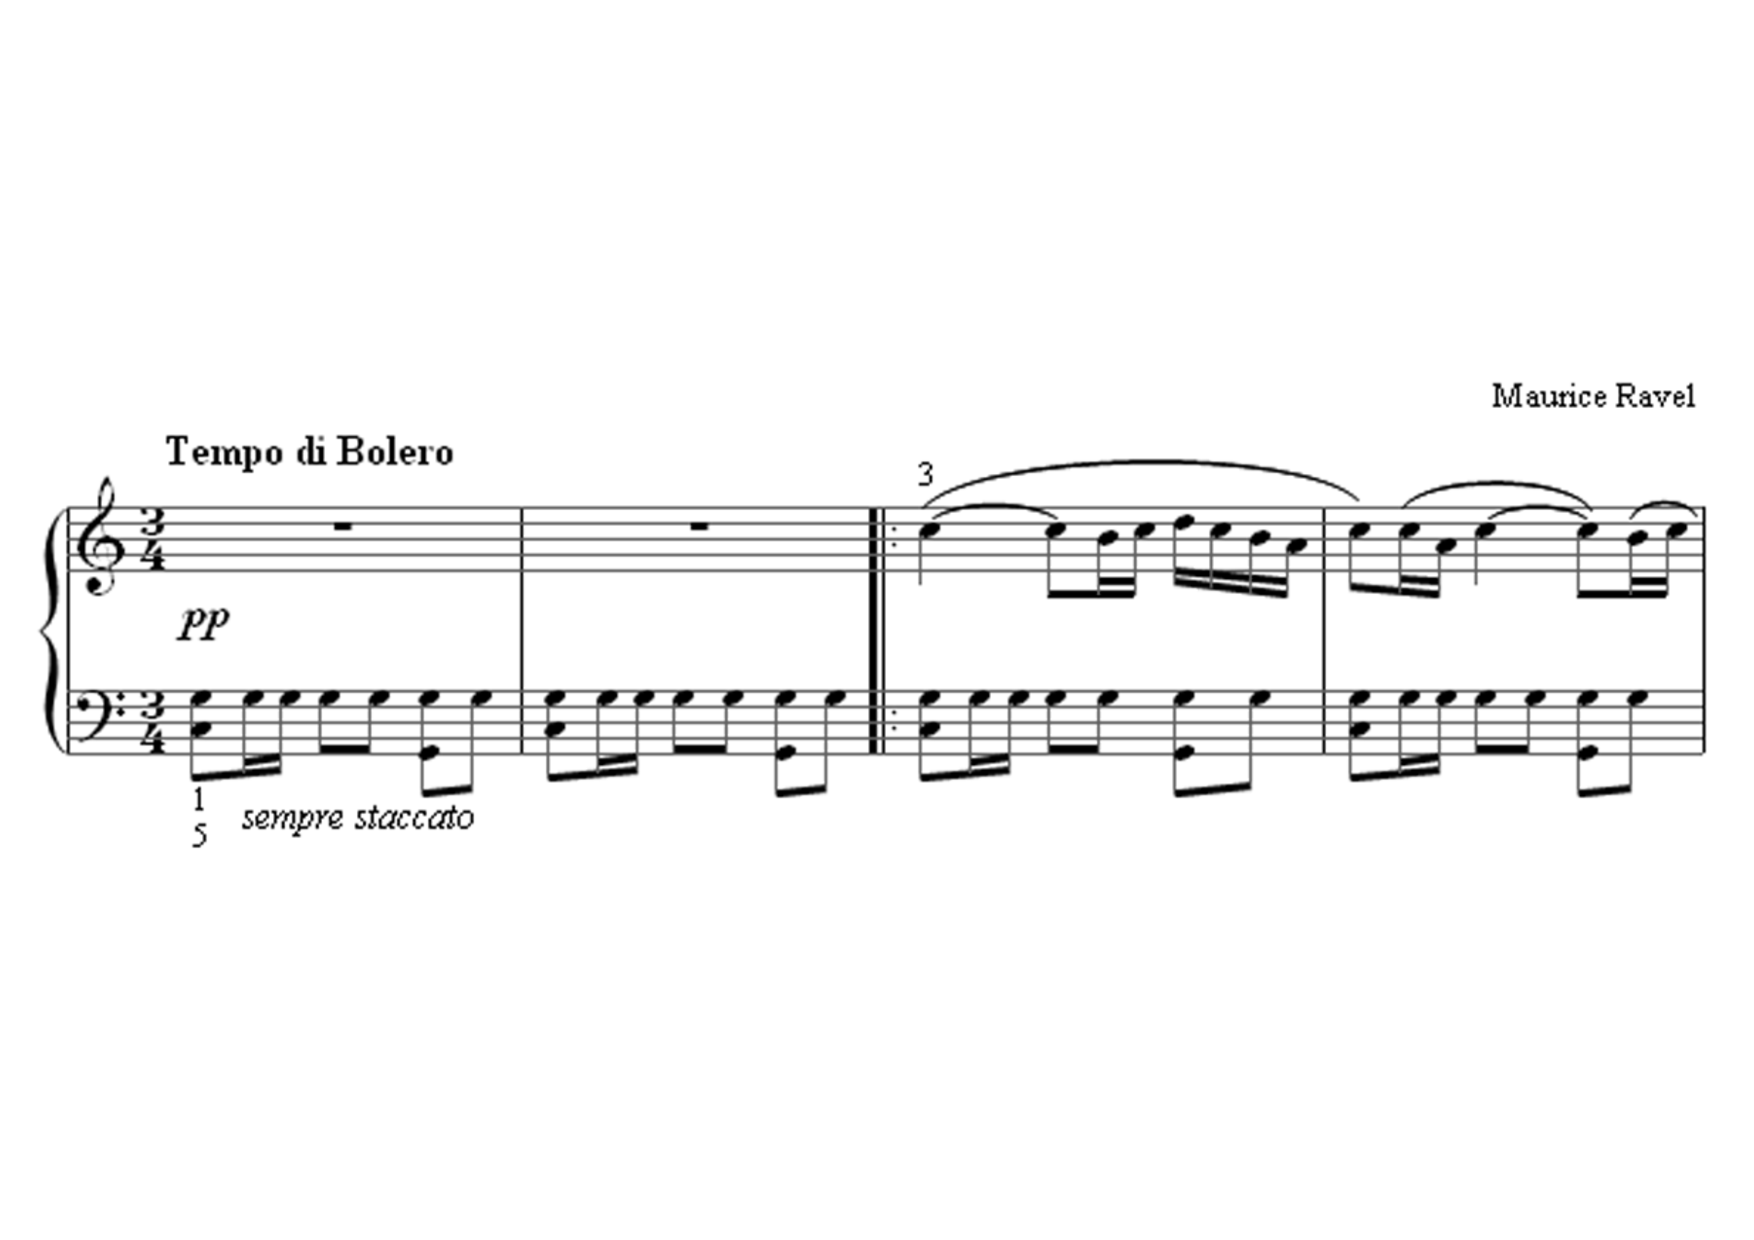
\includegraphics[width=12cm]{figure/Bolero.pdf}
\caption{Ostinato patterns from Bolero's Ravel \citep{Mawer2000TheRavel}}
\label{fig:bolero-ostinato}
\end{figure}

In the Ostinato Model, the phenomena under investigation are modeled as a network, and interactive visualization tools are used to conduct the investigative process. Imperatively, interaction is extended to all the different phases of the analysis process through transparency and the definition of explicit phases. Network analysis introduces a relationship approach to investigating the structure of many kinds of phenomena. Network analysis allows for the exploratory analysis of the social roles of network actors and the complexity of relationships, as well as for quantifying the structural properties of the network representation of the innovation ecosystem under investigation.

A key aspect of the Ostinato Model is the focal point of the user--here, the investigator of an innovation ecosystem--in the investigative process. Putting the investigator to the center of the process answers to the call for data scientists \citep{Davenport2014BigOpportunities}, the almost mythical multi-skilled individuals that are capable of individually running the whole investigative process from collecting data to analysis to deep sensemaking in the domain of interest, by allowing both experts of the domain under investigation, developers of the technical process as well as e.g. quantitative analysis specialists to have equal means to take a proactive role in the investigative process. Moreover, the Ostinato Model defines an overall structure for the data-driven investigative process that supports the coordination between the individual phases of the process and therefore allows all the members of the investigative team to contribute to the implementation of different phases of analysis and, importantly, to the sensemaking on structures and mechanisms emergent in empirical data representing an innovation ecosystem.

The Ostinato Model is developed over a series of experiments in investigating innovation ecosystems with an action design research approach. It is built on existing process models and previous work presented in Figure~\ref{fig:process-model-collage} and it takes into account the process requirements presented in Chapter~\ref{ch:processmodels}. Figure~\ref{fig:ostinato} shows a diagram of the Ostinato Model. Each step is described in the following sections.

\begin{figure}[htb]
\centering
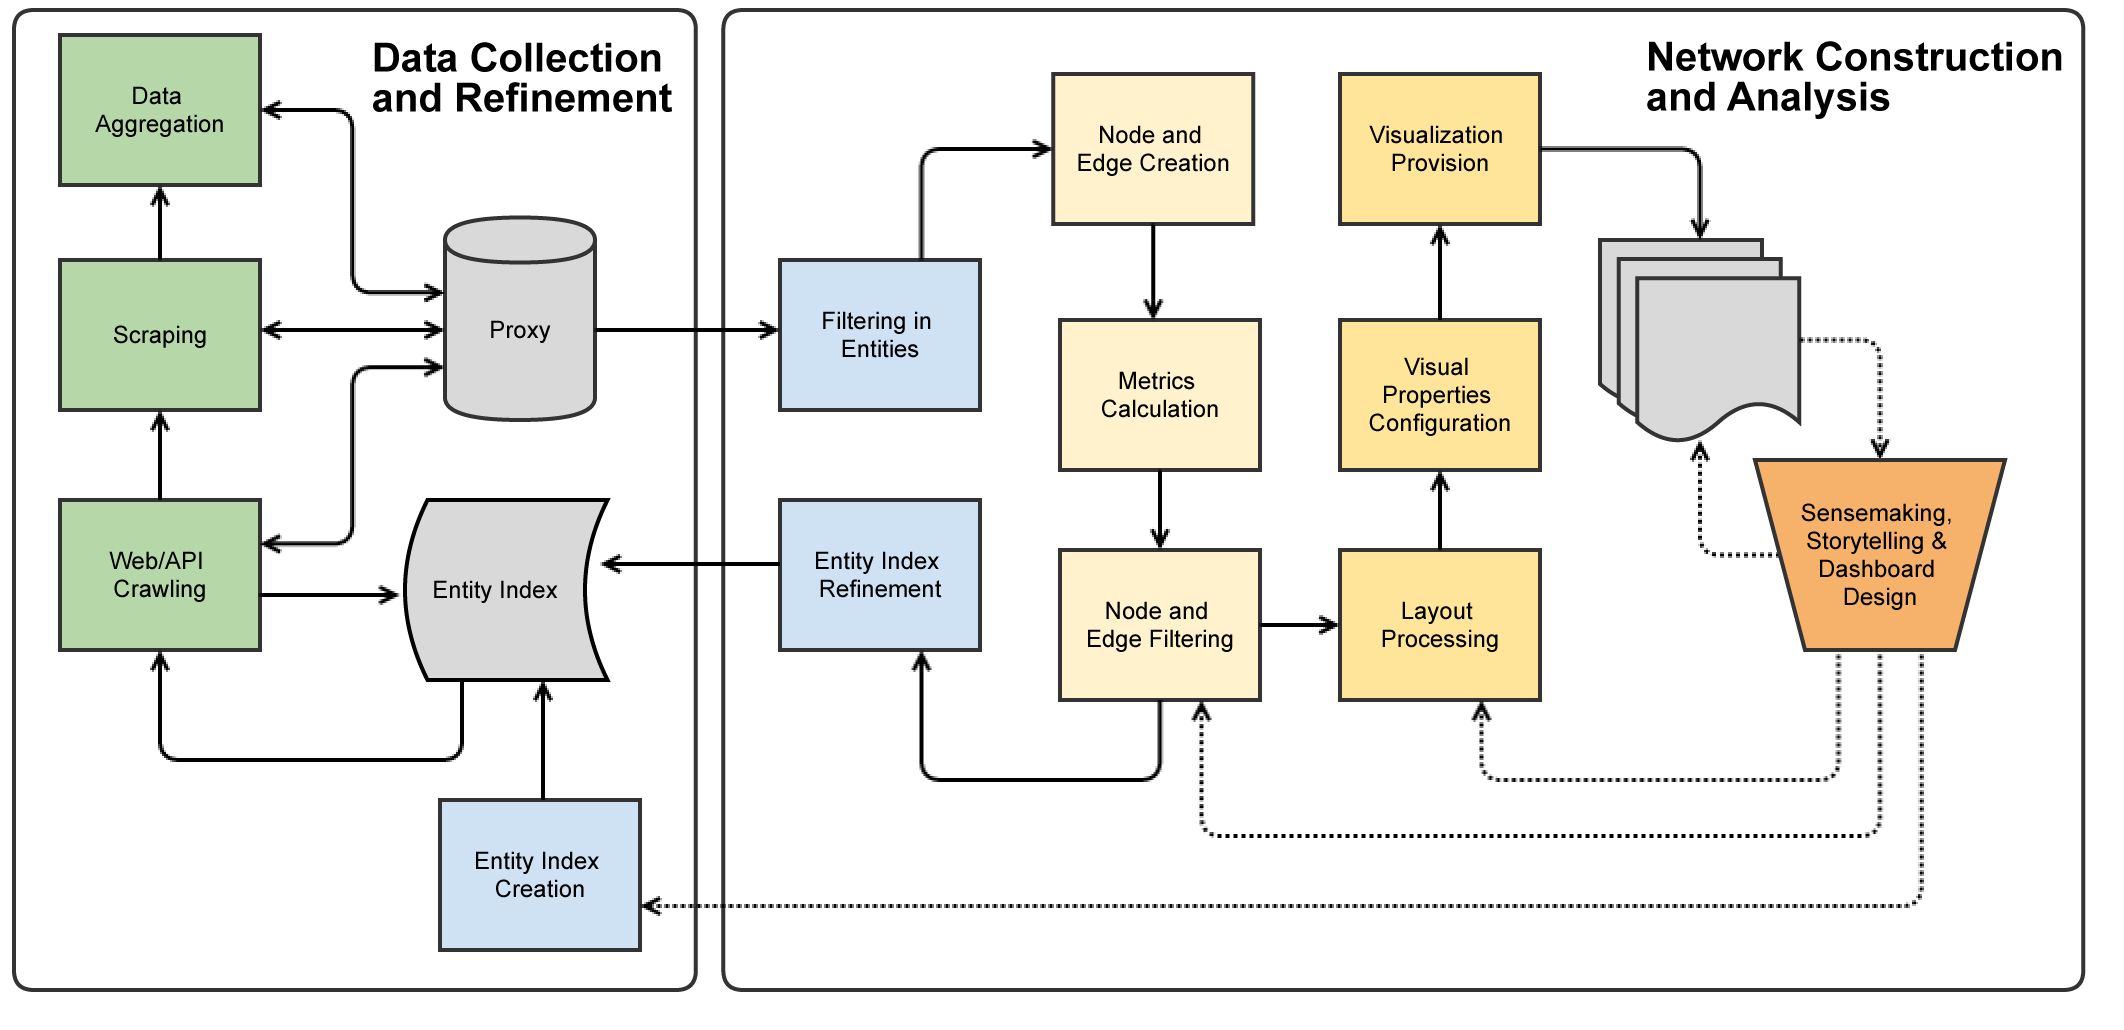
\includegraphics[width=1.0\textwidth]{diagram/kredible_net_process_model-v07.png}
\caption{Ostinato Model--user-centric data-driven process model for visual network analytics}
\label{fig:ostinato}
\end{figure}

Phase 1: Data collection and refinement

\begin{enumerate}
\item Entity index creation
\item Web/API crawling
\item Scraping
\item Data aggregation
\end{enumerate}

Phase 2: Network construction and visualization

\begin{enumerate}
\item Filtering in entities 
\item Node and edge creation
\item Metrics calculation
\item Node and edge filtering
\item Entity index refinement
\item Layout processing
\item Visual properties configuration
\item Visualization provision
\item Sensemaking, storytelling \& dashboard design
\end{enumerate}

\section{Phase 1: Data Collection and Refinement}
\label{subsec:modelphase1}

The general rules of data-driven analytics apply when operating with the Ostinato Model: collecting and cleaning the data will, in most investigations, consume most of the time and resources available for the investigation.

\subsection{Entity index creation}

In some investigations, the source data can be collected in full whereas in others only data on entities that are relevant for the analysis need to be collected. The entities for which data is collected are defined by boundary specification. In investigating the connections between companies taking part in Young Innovative Companies program in \ref{pub:tekesyic}, the list of companies defines the starting point of the analysis \citep{Huhtamaki2012NetworksFinland}. In studying the structure emerging from individual deals and alliances around Google and Motorola Mobility, boundaries are set at two steps from the focal companies \citep{Basole2012UnderstandingApproach}.

\subsection{Web/API crawling}

Collecting the data is the most heterogeneous step in the data-driven visual analytics process \citep[cf.][]{Salonen2013ChallengesMedia}. Possible source data potentially includes everything digital, from proprietary offline documents and document collections to spreadsheets to Web APIs (application programming interfaces) to Web sites that are designed primarily for human interaction. 

Similarly, the functionality required to collect the source data can range from relatively simple reading of individual documents to functions similar to a fully featured Web crawler. Compared to crawling random websites, Web APIs are, by default, more straightforward for data collection as they are often designed to support reuse \citep{Vinoski2008}. At best, source data is available as linked data \citep{Bizer2009}, i.e. data that has a clear structure with individual facts that can be interconnected with the help of unique identifiers to enable referential integrity. 

Thomson Reuters SDC provides a functionality for extracting data on alliances on basis of different search criteria, therefore crawling is not required. Crawling is, however, utilized extensively in collecting the IEN Dataset \citep[see][]{Rubens2010LeveragingMoves}. Moreover, in \ref{pub:tekesyic} we use Twitter REST API for crawling the follower data on companies in Tekes YIC program.

At the end of the crawling phase, a set of web resources, or rather their representations in Hypertext Markup Language (HTML) or some other format, is made available in a local database or other storage, a proxy that significantly speeds up the subsequent processing steps.

\subsection{Scraping} 

Once the raw source data is available locally, the next step is to filter, select and distill the utility data relevant to the analysis process. Scraping refers to the process of distilling data from documents that are published to the Web first and foremost for humans to use. This kind of data extraction and cleaning is sometimes referred to as data wrangling \citep{Kandel2011}. Scraping can further be seen as a form of the Extract, Transform, Load (ETL) process that is often applied in the context of data warehousing or other business intelligence processes to collect data from different sources to be refined and normalized and finally loaded into a consistent database for later use \citep{Petschulat2010,Vassiliadis2009}. 

Scraping-like functionality is required to distill the data from the spreadsheets in Excel format exported from Thomson Reuters SDC. We use JSON to represent the data representing individual deals and alliances. To support non-technical investigators access to the data, the use of CSV should be considered for representing intermediary results for added transparency and lowered entry barrier.

Using Wikipedia data in analyzing the structure of an innovation ecosystem is an example of scraping. When collecting data from Wikipedia on Finnish Young Innovative Companies, for example, the investigators are particularly interested in the facts presented in the Infobox section of the page \citep[cf.][]{Huhtamaki2007CommunityEcosystem}. To collect this data, one can take advantage of the HTML markup on the page to specify the semantics (meaning) of the different pieces of text. Each of the facts is represented as a table row including two cells, the first of which includes the label specifying the type of the fact and the second includes the actual value. Moreover, the value is also represented as a link to a separate page. These pages have to be included in the entity index for crawling and scraping additional facts relevant to the investigation.

\subsection{Data aggregation}

In contrast to data-driven social media studies in which data originates from an individual social media service, the complex context of innovation ecosystem investigations often insists on using several sets of data in parallel. This implies that in most investigations, linked data is not readily available and, therefore, links between individual sets of data have to be constructed through the creation of unique entity identifiers that allow referential integrity. 

In innovation ecosystem investigations, the name of the company or another actor is sometimes the key data point that can be used to identify an entity. In \ref{pub:multiscopicfinland}, we use actor names to find entities that appear in more than one dataset. To take into account differences in the spelling of the names, we apply OpenRefine\footnote{OpenRefine is an open source tool for working with messy data, \url{http://openrefine.org/}} to harmonize the names through a semi-manual process. In studying whether co-author networks show small-world properties, \cite{Newman2001TheNetworks} uses author names with and without additional initials to create upper and lower bounds for network measurements. String matching \citep{Navarro2001AMatching} and named entity recognition \citep{Finkel2005IncorporatingSampling} are examples of machine learning-based methods to support automation for creating unique identifiers for actors. 

\section{Phase 2: Network construction and analysis}
\label{subsec:modelphase2}

Once the data is available in a local proxy, the utility data has been extracted from the source documents, and data from different sources has been aggregated into a consistent set of linked data, the construction of the network representation of the innovation ecosystem under investigation can begin.

\subsection{Filtering in entities}

The network construction phase starts with a selection of the entities to be included in the network. The selection of nodes is guided by the boundary specification designed and defined by the investigative team. At least two approaches exist to implement the selection: starting from a list of entities and rule-based entity inclusion.

To continue the Finnish YIC example in \ref{pub:tekesyic}, we start from the list of companies participating in the program and continue to include all the individuals and investors directly connected with the company. Moreover, we include companies that are connected to the companies already in the sample through an investment or acquisition. For investigations on the Finnish innovation ecosystem and EIT ICT Labs in \ref{pub:multiscopicfinland} and \ref{pub:eitictlabs}, respectively, companies are selected on basis of their location. In both investigations, directly connected companies, individuals and investors are included in the sample.

A key reason to separate the selection of entities from node and edge construction is to support the transparency, reproducibility and extensibility of the process. To create a shared understanding of the results of the analysis, it is absolutely vital that all the investigators taking part in a particular network investigation are able to access and understand the original raw data, in addition to any constructed variables, and the various analytics and metrics that represent the network; this means that investigation participants need access to data from raw to refined. According to our experience, answering specific questions raised by anyone interested in an investigation, drawing conclusions, generalizing the results, developing more specific and potentially more interesting questions all depend on transparency of the data available and used for the analysis.

\subsection{Node and edge creation}

Creation of the network is of course a core part of the data-driven network analysis process. Network creation boils down to the creation of nodes representing the actors and the creation of edges representing the connections between the actors. Several options are, however, available when specifying details of the network creation process. First, the network can be either one-mode or two-mode. In one-mode networks all the nodes are of same type: startup companies or investors, for example. Connections between the nodes are formed through relationships: investments, affiliations to individuals, acquisitions and transactions. In two-mode networks, there are two types of nodes, for example, startup companies and individuals related to them. Hypergraphs and bipartite graphs are examples of means to visualize two-mode networks \citep{Jesus2009,Freeman2009MethodsVisualization}.

Further, the connections between network nodes can be either weighted or dichotomous. The strength of a connection can be expressed with weighted connections. In either case, the connections may be undirected or directed. Moreover, temporal dimension can be included in networks if the data used to create the connections is time-stamped. As we show in \ref{pub:demola} and \ref{pub:mobileecosystem}, with temporal data, insights about the evolution of the network can be provided.

In all of the investigations included in this dissertation, we have eventually decided to use multimodal networks for representing the innovation ecosystems under investigation. We assume that the main reason for this is the exploratory, descriptive nature of the investigations that highlights the importance of the system-level view over detailed measurement of structural properties. 

\subsection{Metrics calculation}

Network metrics enable quantifying a variety of structural properties, both in network and node level. These range from simple metrics such as node degree (indegree, outdegree) \citep{Freeman1978CentralityClarification} and betweenness to PageRank \citep{Page1999TheWeb} hub and authority values with HITS \citep{Kleinberg1999AuthoritativeEnvironment} and other more sophisticated measures. Whereas in principle, every metric can be calculated for all of the networks and their nodes, in practice this is not always feasible due to reasons of efficiency. Moreover, new metrics for networks are being developed continually, and the investigative team is likely to find--or develop--new metrics that fulfill specific investigative purposes. From an implementation viewpoint, it is unlikely to find one tool that supports all the metrics the team wishes to use. Therefore, a combination of tools may be required to calculate the metrics. Loose coupling allows this.

As part of metrics calculation, network metrics for the network representation should be stored for later usage. For transparency, a list of exported network nodes and edges should include the various metrics used. In practice, node and network metrics must be recalculated after each change in the network structure; however, reference to previous calculations is often needed e.g. for analyzing the change in the structural position of nodes.

The selected network structure dictates the metrics that can be calculated for the network and individual nodes. A one-mode network that has directed and weighted edges allows using the widest range of node and network metrics. In a multimodal network of companies, investors, and individuals, for example, metrics such as density or authority may not be fully relevant as e.g. investors can never be connected to other investors if the connections are based on investments.

\subsection{Nodes and edge filtering}

A key limitation of visual network analysis is the amount of space available, both on screen and particularly on paper, to present the visualization. Depending on the level of detail required in the analysis, hundreds or thousands of nodes can be presented in one visualization view. For networks of tens of thousands of nodes and more, only more general structures and patterns can be observed from a visualization. 

Two means exist to address this limitation: the best option is to allow the visualization users to filter in and out nodes and edges. If the end-user tools used to present the visualizations do not allow filtering, it can be done as one part of the automated process. Often, reducing the size of the visualized network is accomplished with a combination of filtering out edges that have the least amount of weight as well as filtering out nodes that: 1) are left without edges; 2) have a value of the degree or some other a network analysis metric under a specified threshold; or 3) are (not) of particular type (even though this can already be taken into account when filtering in the entities used to construct the network in the first place).

\begin{figure}[htb]
\centering
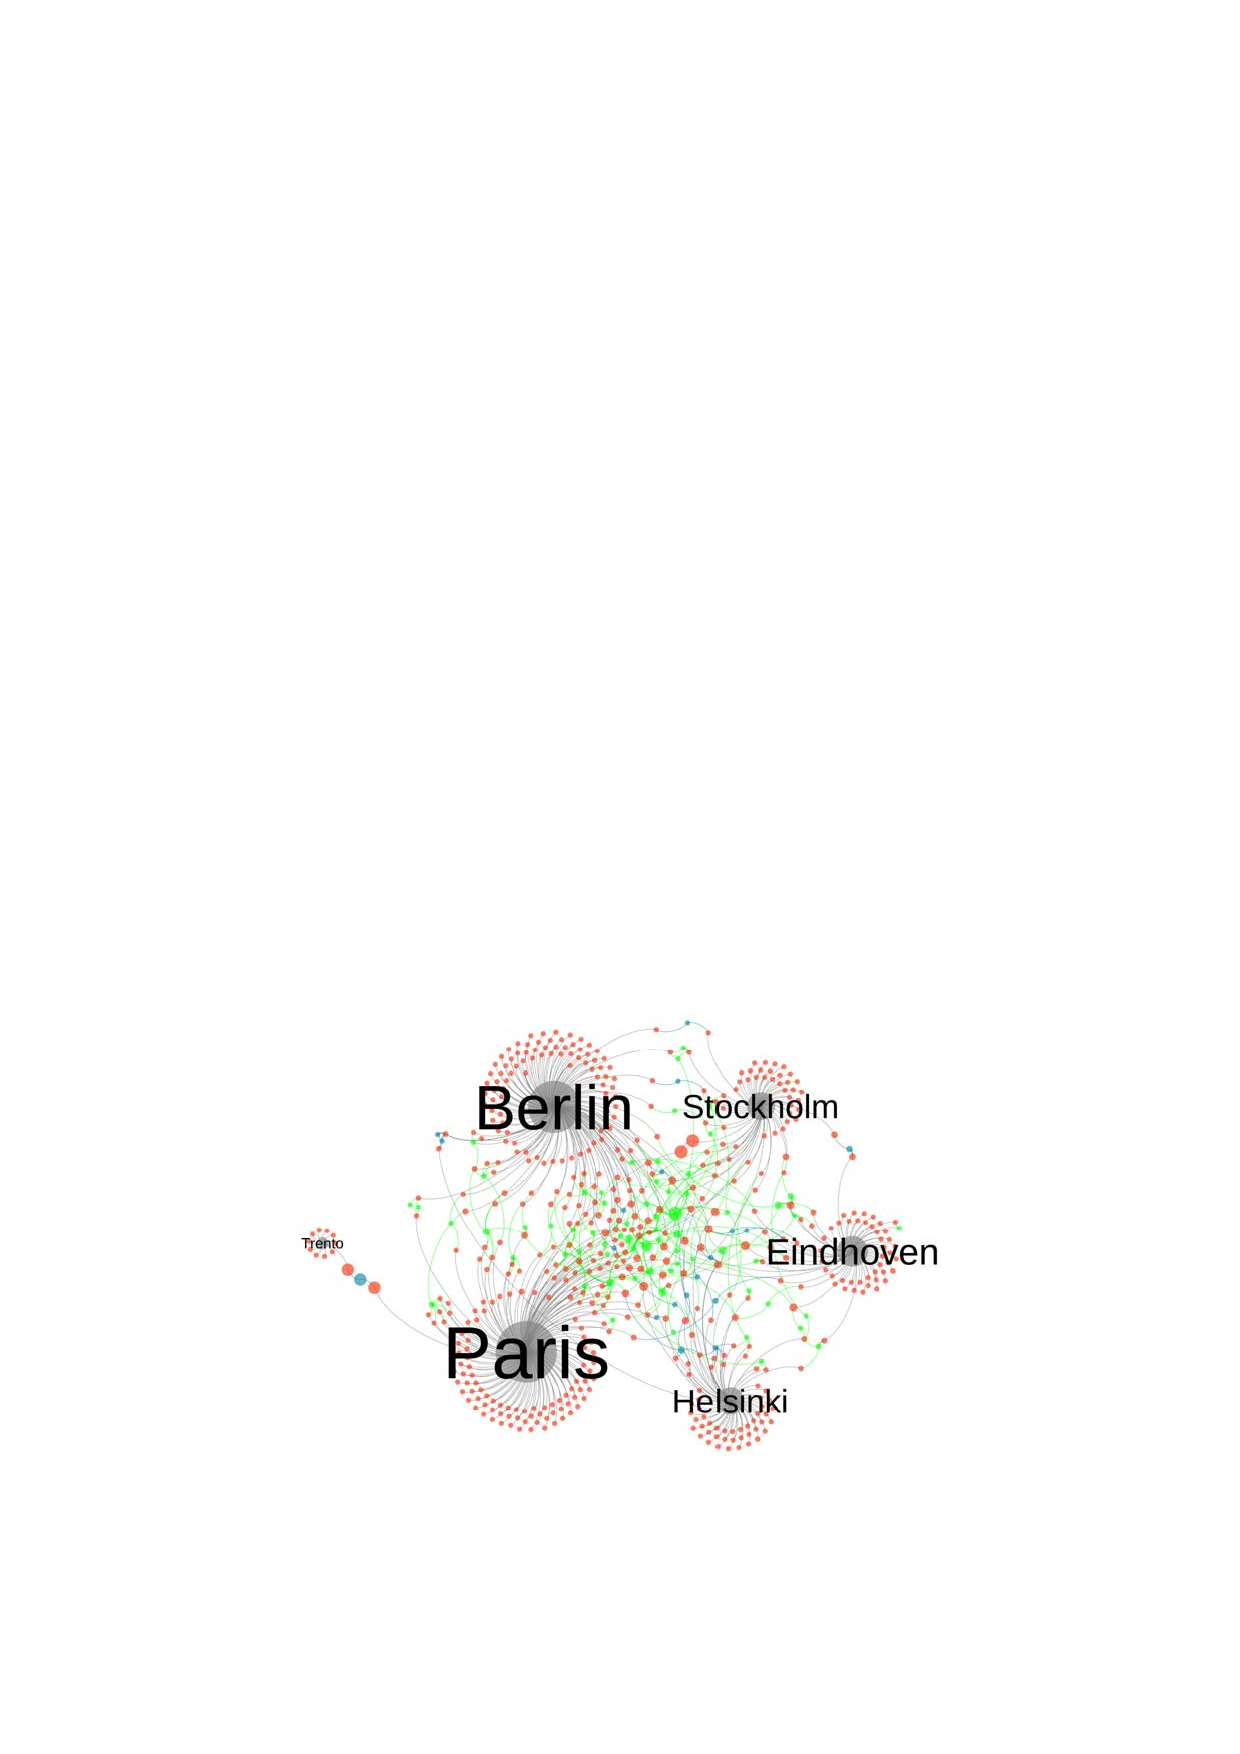
\includegraphics[width=12cm]{figure/eitictlabs-top10percent.pdf}
\caption{Top 10\% of individual, companies and investors connecting EIT ICT labs co-location cities according to their betweenness. The role of venture capital investors as enablers for mobility becomes evident.}
\label{fig:eitictlabs-top10percent}
\end{figure}

In Figure \ref{fig:eitictlabs-top10percent} in \ref{pub:eitictlabs}, we provide a filtered version of the network structure of EIT ICT Labs to highlight the importance of venture capital investors in connecting the different co-locations centers and therefore in enabling mobility in Europe. The nodes are filtered in according to their betweenness centrality. In \cite{Jarvi2016DismantlingLinkages}, we apply filtering to investigate innovation ecosystem by dismantling ``the network structure through a procedure that resembles peeling an onion.'' 

\subsection{Entity index refinement}

At this stage of the process, the network representation of an innovation ecosystem under investigation is constructed and the required metrics are calculated for each of the nodes. Depending on the boundary specification applied in the investigation, the network is either ready to be visualized or, alternatively, additional data can be collected to complement the network. Revisiting the Finnish Young Innovative Companies case in \ref{pub:tekesyic}, the boundary specification is designed to include all the individuals involved in one or more of the companies in YIC program as well as all the other companies the individuals are or have been affiliated with. Moreover, the data includes all the investors that have invested into any of the companies as well as all the companies that have acquired any of the YIC companies.

Entity index refinement has a particularly important role when using multiple sources of data. If, for example, boundaries of the innovation ecosystem under investigation are set to two steps from the focal companies, the actors coming in through the first step should be taken into account across datasets.

\subsection{Layout processing}

The principle of processing network layout is simple. Nodes are given a position in two-dimensional space in a way that network structure is revealed in an expressive, intuitive way. Despite the simplicity, novel layout algorithms have been developed over several decades.

In the investigations included in the dissertation, various stakeholders found a specific implementation of force driven layout, Force Atlas, to be particularly suitable for laying out networks representing innovation ecosystems at different levels. In fact, Force Atlas is used in all the investigations included in this dissertation. Force Atlas is implemented in Gephi \citep{Bastian2009Gephi:Networks} and can be used as a batch process with the help of Gephi Toolkit\footnote{Gephi Toolkit, \url{http://gephi.github.io/toolkit/}}. 

In practice, the parameters of the layout algorithm must be adjusted manually for a particular kind of a network before fully automating layout processing. Alternatively, the layout can be processed with the user interface version of Gephi and the resulting network, including the X and Y coordinates for each node, can be exported as part of the network representation in GEXF or other suitable format.

Storing the network layout data is particularly important for improving the efficiency of the analysis process, as well as for reducing investigators’ cognitive load and for promoting transparency. In particular, it is important that after the data is refreshed, the investigators are able to find the pre-existing nodes in an area of the network where the nodes were previously located. This stability can be achieved by inserting the existing positions into the network data before re-running the force driven layout algorithm. In most cases, investigators will find the pre-existing nodes close to the initial area of the network.

Future work is needed to determine how features such as layout algorithms, e.g., those implemented into NodeXL, could be used as a component of data-driven visual network analysis pipelines. 

\subsection{Visual properties configuration}

There is a limited set of possibilities for defining the visual appearance of a network. Nodes have size, color and perhaps a border and shape as elected visual features. Edges have color and width.

Both node and edge properties originating from the source data as well as node metrics can be used to define the visual properties of nodes and edges. In our investigations, node size in most cases represents its betweenness centrality and node color the type of the actor it represents. At best, visual properties are defined as part of the automated pre-processing routines instead of selected manually e.g. in Gephi.

Allowing the user of the visualization to select and change the visual properties according to node metrics and other node properties is perhaps the easiest way to allow end user interactivity in network analysis. Depending on the tools used by the investigators to conduct the analysis, the visual properties of nodes and edges can continue to be tweaked as part of the interactive analysis process.

\subsection{Visualization provision}

At this stage, a network has all the required information available and therefore can be visualized. The means to finalize this step depend greatly on the tools that have been selected for use by the investigative team. In most cases, however, the created network is serialized into a file following a selected vocabulary or format for representing a network. These vocabularies and formats range from different CSV based applications to XML-based languages designed for representing networks.

A minimum approach to provision the network visualizations is to export network data in GEXF or other suitable format and place the resulting file into a folder from where a library such as Gexf.js can access it. More generally, viewer composition scenarios can include the following:

\emph{Scenario 1}. Network viewer component with fixed functionality, i.e. following a fully descriptive approach. Visual properties such as node size and color need to be defined into the data during its processing. Gexf.js is an example of such a component that we have found useful in adding value to a fully static PDF-based approach in disseminating network visualizations.

\emph{Scenario 2}. Implementing a dashboard with Web technologies, more specifically frameworks such as Highcharts, D3.js, Crossfilter.js, DC.js and others. In this case, tailored interactive features for data exploration can be provided to the user, adding options for representing network data. 

\emph{Scenario 3}. Using full-feature explorative analytics tools such as Gephi, NodeXL and Tableau, which can be used to further process the data and to connect source data to visual properties of the visualization. The key here is to produce visualizations rich-enough in data that the analyst can fully utilize the critical properties of the chosen analytics tool for investigation and exploration. In Gephi, for example, it is useful to include attribute data for nodes to assist network filtering in a way the investigator desires to do.

\subsection{Sensemaking, storytelling and dashboard design}

While information visualization includes data transformation, representation, and interaction, it is ultimately about harnessing human visual perception capabilities to help identify trends, patterns, and outliers. Sensemaking has its roots in cognitive psychology and many different models have been developed. Sensemaking procedures are cyclic and interactive, involving both discovery and creation \citep{North2006}. During the data collection and refinement phase, an investigator searches for representations. In the network generation phase these representations are instantiated, and based on these insights the representation may be shifted, to begin the process again. Sensemaking is closely linked to the insight objectives \citep{Konno2014}, and the Ostinato cycle of exploration–automation is key in achieving actionable insights that innovation ecosystem investigators, analysts, and orchestrators can utilize.

When sensemaking requirements are satisfied for investigators and other users, steps of the Ostinato process can be formalized with automated procedures for iteration over time. Key actors, relationships and events of the network can be incorporated into dashboards that will track changes in critical assumptions and into stories that will share vision for actionable change.

\section{Utility and added value of the Ostinato Model}

In this dissertation, Ostinato Model, a new process of data-driven visual network analytics is developed and described. The Ostinato Model contributes to the call for more expressive means for supporting innovation ecosystem investigations in two ways. First, it can be applied to support the data-driven investigations of innovation ecosystem structure and dynamics. Second, for validity and reliability of these investigations, it is key to increase the transparency of the processes behind the data originating from various digital sources.

Moreover, the Ostinato Model contributes to the data-driven network investigations of innovation ecosystems in three different ways. First, the network approach has great strength in supporting the exploratory investigations of the patterns in between actors of innovation ecosystems. Second, referring specifically to the first phase of the Ostinato Model, data-driven approach allows tracking down processes over the boundaries of individual sources of innovation ecosystem data. Third, user-centricity of the data-driven process adds to the transparency of the process itself, therefore providing means to triangulate different phases of data refinement and transformation and allowing different stakeholders of investigations to take as proactive role as they wish in moving forward a particular investigative process.

Due to the continued and rising interest in big data analysis, new tools are continually introduced to support investigative work. Despite the development of all-in-one tools, a combination of tools is likely to continue to provide more flexibility in accessing and aggregating data and in processing and analyzing it. Finding a balance between user interface-operated low barrier tools and expressive computational strategies that require technical knowledge is key in making the investigative process as productive as possible while maintaining transparency and process flexibility.

The proposed Ostinato Model for user-centric, process-automated, data-driven visual network analytics meets many of the requirements outlined in \ref{sec:processmodelrequirements} for the exploration–automation cycle recommended for developing shared understanding.

Using files rather than databases for representing intermediary results supports both loose coupling and transparency of the process. It also allows for implementing some of the steps manually, if seen feasible, and the flexibility of the process in general is increased.

Allowing exploration boils down to the selection of the end user tools for investigators to visualize and explore the data. If a rather static tool such as Gexf.js, for example, is used, the user is limited to browsing and searching the data. If importing the data into an exploration platform such as Gephi or NodeXL is permitted, it is possible to provide the user with rich node and edge data, enabling them to continue their explorations with more independence. The availability of expressive visual analytics tools, such as Tableau, adds to investigation options of analyzing network data, either as a network or using node and edge level data to provide new inspirations for other kinds of data analyses.

Low entry barrier is enabled through making intermediary results available to all the members of the investigative team. As the process is repeatable and its individual steps are automated, new projections of the data can be implemented in an iterative and incremental manner. Implementing completely new steps of analysis becomes possible even without technical skills. Automating the steps, however, requires developers’ attention. The Ostinato Model requires a multidisciplinary data science team or the somewhat mystical multi-skilled data scientist \citep[cf.][]{Davenport2014BigOpportunities} to conduct the investigation.

Interoperability can be built into the computational approach. This requires that the technical architecture is flexible enough to permit different software components and tools--that may be implemented with different technologies--to be introduced into the process. When an analysis pipeline is built completely from scratch, it is recognizably important to minimize the number of technologies used. However, moving fast and in an agile manner is an objective we claim can be achieved when existing tools can be integrated into the pipeline to implement the individual steps of the analysis process and to provide the visualizations to investigators and other end users.

Reproducibility is both a technical and a policy requirement. For an investigative team revisiting or extending an existing investigation, the availability of runnable code, source data, and intermediary results provides a fruitful starting point. Moreover, the results of reproducible studies can be published in a way that both data and runnable code are available, providing a solid foundation for others to add their contributions as well. A reasonable proposition is that such a piece of knowledge draws attention from other researches and therefore has increased potential for impact. Automation is a key requirement in reproducibility, as well as in creating dashboards that continues to update visualizations of the phenomenon under investigation, sometimes in close to real time.  

Setting up persistent data-collecting routines requires, in general, a programmatic implementation and must be designed and implemented case by case. To maintain the transparency of the process, it is important that the investigators are able to access both the raw data as well as to track down the individual steps used to derive the data that is eventually used for the analysis and visualizations.

More generally, an implementation of the Ostinato Model can serve as the core engine of an investigation. It can also be used to develop a pre-processing pipeline that collects and refines the data, creates a network representation and serializes the outputs to be analyzed and processed with expressive tools that, standing alone, allow the full visual analytics cycle for users. 

A key challenge of the presented approach concerns the number of options for investigators and other end users to interact with the data in real-time while conducting the analysis, particularly the non-technical investigators on a multi-disciplinary team. The action design research approach favors an iterative approach for both data-driven explorations and evidence-based decision making. However, investigators with limited programming skills or related technical know-how are limited in their participation, even though they may possess vital domain intelligence. Through access to data, documentation of changes in the analytical approach, flexible means to produce network representations in various formats, and exposition of intermediary results, barriers to participation are lowered. The cycle of exploratory visual analytics, confirmation of data selection rules, and analytical results made accessible through high interactivity visual analytics, allows the investigative team to confirm assumptions and investigative procedures, identify aspects of the analysis that can be automated and establish a transparent, reproducible process.